% !TeX root = ../main.tex
% Add the above to each chapter to make compiling the PDF easier in some editors.

\chapter{Implementation}\label{chapter:implementation}

As explained in \autoref{sec:terminology}, from now on the term Firmware ID (FWID) will be used instead of the previously used term TCB Component Identifier (TCI).

\section{Overview}


We run our implementation on ARM's Fixed Virtual Platform~(FVP)\footnote{\url{https://developer.arm.com/Tools\%20and\%20Software/Fixed\%20Virtual\%20Platforms}} which is a complete simulation of the Armv8-A architecture including TrustZone.

To do this, we use the software infrastructure provided by OP-TEE for various platforms, including FVP\@.
OP-TEE uses the TrustedFirmware-A~(TF-A)\footnote{\url{https://www.trustedfirmware.org/projects/tf-a/}} package from ARM as firmware boot components.
However, we mock their attestation, i.e., their Alias certificates are statically compiled into the binaries instead of being dynamically generated, as TF-A does not implement DICE\@.
The development efforts to implement that exceeds the benefits, as the concept can also be demonstrated with mocked certificates.
For that, only the certificates up to the OP-TEE~OS are mocked, including OP-TEE~OS's private key to sign the subsequent Alias certificate, which is our EKcert.

Our implementation with compilation and running instructions can be found on GitHub\footnote{\url{https://github.com/akorb/master-thesis-meta}}.

\section{Boot chain}

The boot process is depicted in \autoref{fig:boot_chain}.
DICE is the root of trust, because incorrect behavior remains undetected and would jeopardize the security of our attestation process.

\begin{figure}[htpb]
  \centering
  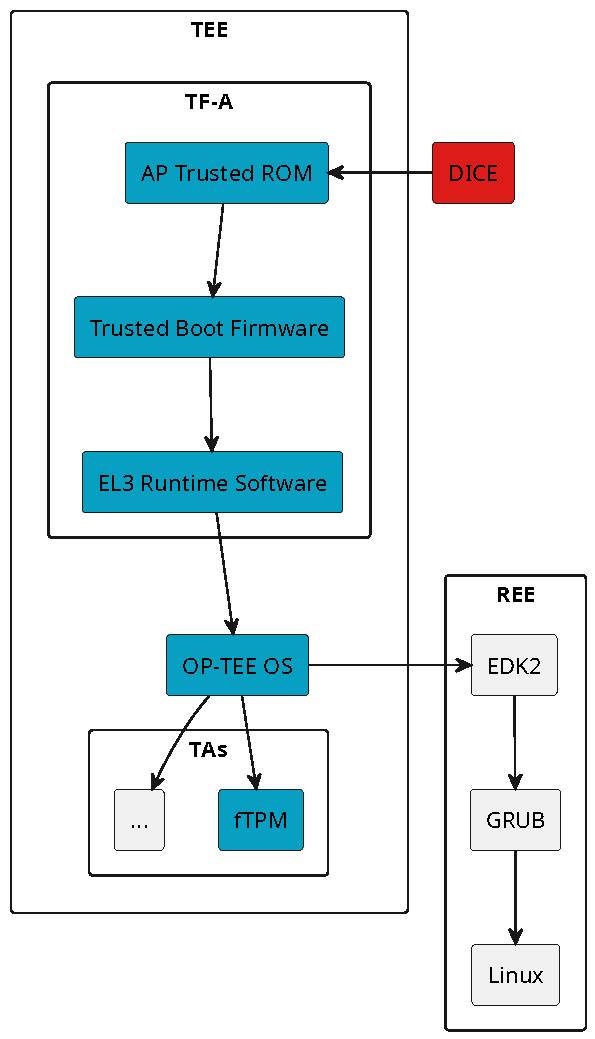
\includegraphics[width=0.8\linewidth]{figures/boot-chain.pdf}
  \caption{The boot chain of our system running in Arm's FVP\@. Blue: Represented by our yielding certificate chain. Red: Root of trust for verifier, and assumed to be present.}\label{fig:boot_chain}
\end{figure}



\paragraph{DICE}
Theoretically, the boot chain begins with the DICE hardware, but this is not included in FVP\@.
Therefore, we simply assume its presence by mocking the first few certificates of the yielding certificate chain.
Furthermore, it is independent hardware, and therefore, neither part of the TEE nor the REE\@.

\paragraph{TF-A}
After reset, the CPU executes within the secure world.
That is also the reason why machines that are unaware of the separation between secure world and normal world are running in the secure world, as they never modify the execution environment of the processor.
This also ensures that TrustZone unaware systems have all expected privileges, which would be restricted in the normal world.
The Application Processor~(AP) Trusted ROM sets up the platform-specific exception vectors.
The Trusted Boot Firmware enables the MMU, performs the platform security setup, and other tasks.
The final component of TF-A --- EL3 Runtime Software --- replaces the simple and rudimentary initialization performed by the AP Trusted ROM with more complete configurations by detecting the system topology, and enabling normal world software to function correctly.
The EL3 Runtime Software also provides the monitor which conducts the context switches between the secure world and the normal world.
More complete and detailed information can be found in the TF-A documentation\footnote{\url{https://trustedfirmware-a.readthedocs.io/en/latest/design/firmware-design.html}}.

\paragraph{OP-TEE~OS}
Finally, the OP-TEE~OS\footnote{\url{https://github.com/OP-TEE/optee_os}} is loaded and executed.
Just like an ordinary operating system, it initializes its functions offered to the user space of the secure world, i.e., the trusted applications.

\paragraph{Trusted Applications}

Our TA in focus is the firmware TPM\footnote{\url{https://github.com/microsoft/ms-tpm-20-ref/}}\@.
It consists of the reference code by Microsoft which implements a TPM, and the stub code, which provides and implements the interfaces required to be a TA of OP-TEE\@.
This fTPM only allows a single connection at any time, i.e., it prohibits concurrent access as this could lead to inconsistent states.
This also mirrors hardware TPMs, which are usually attached via serial buses like SPI to the processor.
Typically, the only entity that communicates with the fTPM is a Linux kernel module\footnote{\url{https://docs.kernel.org/security/tpm/tpm_ftpm_tee.html}}, so it is transparent to the user applications whether the TPM is implemented in firmware or hardware.
Note that TAs are not started automatically.
In fact, we are not aware of any function provided by OP-TEE~OS to register a TA to be started during the boot process. 
Instead, TAs are initialized the first time someone wants to interact with them.

\paragraph{EDK2}
TianoCore EDK II\footnote{\url{https://github.com/tianocore/edk2}} is the first component launched in the normal world.
It is a reference implementation of UEFI~\cite{UEFI} by Intel.

\paragraph{GRUB}
The GNU GRand Unified Bootloader\footnote{\url{https://www.gnu.org/software/grub/}} is a bootloader which is responsible for loading and transferring control to OS kernel software.

\paragraph{Linux}
As expected, the final component to boot is the Linux\footnote{\url{https://www.kernel.org/}} operating system.

\section{Firmware TPM initialization}

% Formula from https://trustedcomputinggroup.org/wp-content/uploads/Hardware-Requirements-for-Device-Identifier-Composition-Engine-r78_For-Publication.pdf
\begin{equation}
  EPS = HMAC(CDI,\ ``EPS'')
\end{equation}

Generate EK with \texttt{TPM2\_CreatePrimary}.

Create EKCert with EKPub as subject signed by OP-TEE private key containing the hash of the fTPM TA\@.
Only memory that is executable, i.e., does not change.
% Add notion.so notes


% Use the attributes for the NVindex of the EKcert as defined by TPM PC Client Spec 4.5.2.1
% The attributes set such that the NV index can only be written or deleted if the policy is fulfilled. However, it has an empty policy, which can never be fulfilled. This yields an undeletable EK certificate.

% \section{Providing a custom EK template}
\section{Adaption of the Endorsement Key}

The EK is a primary key, so it is derived from the Endorsement Primary Seed (EPS).
There is also a default template defined by TCG~\cite{tcg-ek}, dictating the endorsement key to be a restricted encryption key, since it is privacy-sensitive.
The default template is required to be able to reproduce the EK contained in the EK certificate so that the TPM can prove that this EK certificate corresponds to it by being able to generate the corresponding private key.
The default template is not stored on the TPM, but it is part of the command triggering the key generation (\texttt{TPM2\_CreatePrimary}).
Therefore, the TPM itself does not need to know what the default template is, since it is always provided by TPM-capable software.

However, we want to use the EK as a signing key.
The TPM specification provides a mechanism for this, where we need to store our custom EK template in a specific NV index within the TPM~\cite{tcg-ek}.
We use the values of the default EK template and only deviate from it when necessary in three aspects.
We declare the EK as a (i) restricted signing key.
This also requires to specify a (ii) signature scheme, and (iii) no inner symmetric key as required for signing keys since they are not allowed to have any children keys.

This template will be generated within the TPM after each manufacturer reset, so it will be preserved even after an identity change and a reset of the firmware TPM\@.
However, the EK itself will change as the CDI changes, then the EPS and finally the EK\@.
The attributes of the NV index are declared such that the template cannot be deleted~\cite{tcgPcClient}.
This is possible by allowing to delete the NV index only when an unfulfillable policy is met.

% Ensure that the template generated by code is also directly used, instead of indirectly via unmeasured storages.
The NV storage is not attested since it's ``working data'' and not ``configuration data'', and would be hard to attest since it's encrypted and the cipher text often changes since the IV is generated randomly on each store.
However, the component right before the fTPM knows the fTPM's CDI, could generate the according symmetric key to decrypt the NV storage, and integrate the required NV values in the TCI\@.
By baking the EK template generation in code which is already attested (and the code exists anyways), we prevent this complexity.

The ``working data'' is not attested, since this would restrict the functionality of the fTPM\@.
So, the an NV index is with ordinary TPM commands, providing the required policy/authentication is fulfilled.
We consider this configuration as out-of-scope for attestation, for the former mentioned reason.
In other words, it could be that everyone can change the NV index, where the template is stored.
And in the subsequent boot, we would create a EKcert for it, without anything.
Therefore, during EKcert creation, generate the template in code (which is attested), and use this directly.

% 5.3.2 from https://dl.acm.org/doi/10.1145/3098954.3103165
% Use the references there to explain why we used HMAC with SHA256
% Even though https://trustedcomputinggroup.org/wp-content/uploads/Hardware-Requirements-for-Device-Identifier-Composition-Engine-r78_For-Publication.pdf says hash-only is also an option, https://nvlpubs.nist.gov/nistpubs/SpecialPublications/NIST.SP.800-57pt1r5.pdf (Table 3) shows that the HMAC version has roughly double security strength. Cite all three here (ACM, TCG, NIST)!

% Derivate secrets from CDI
% Used HMAC as recommeded by TPM Hrdware spec

% Attestation PTA hashes calling TA, not arbitrary TA

\section{Prover}
\subsection{Normal World}

\subsection{Secure World}

\subsubsection{Measuring the fTPM}

\section{Attester}

\section{Times}

Usually, the notBefore time of Alias certs should be build time, and notAfter should be infinite.
Network-enable our FVP, but heavy setup for simple demonstration of our system.
Could malfunction sometimes because of time dependencies.
To keep our system easily understandable and simple to access a demonstration, we use fixed times.

% List datetimes of all certificates and FVP system time
% Maybe in a graph with timeline

\section{Technical obstacles}

We would have liked to use RSASSA-PSS which is formally proven to be secure over RSASSA-PKCS1-v1\_5.
RFC 8017 even requires RSASSA-PSS for new applications~\cite{Moriarty2016}.
However, it is not fully supported by the tpm2-tools, yet\footnote{\url{https://github.com/tpm2-software/tpm2-tools/issues/3283}}.
